\begin{figure}[h!]
    \centering
    \caption{Changes in the minimum wage measures under counterfactual
             minimum wage policies, Chicago-Naperville-Elgin CBSA}
    \label{fig:map_chicago_cf_wkp_res}
    
    \begin{minipage}{.95\textwidth} \centering
        Panel A: Increase in federal MW from \$7.25 to \$9
        \vspace{1.5mm}
    \end{minipage}

    \begin{subfigure}{.4\textwidth}  \centering
        \caption*{Changes in residence MW}
        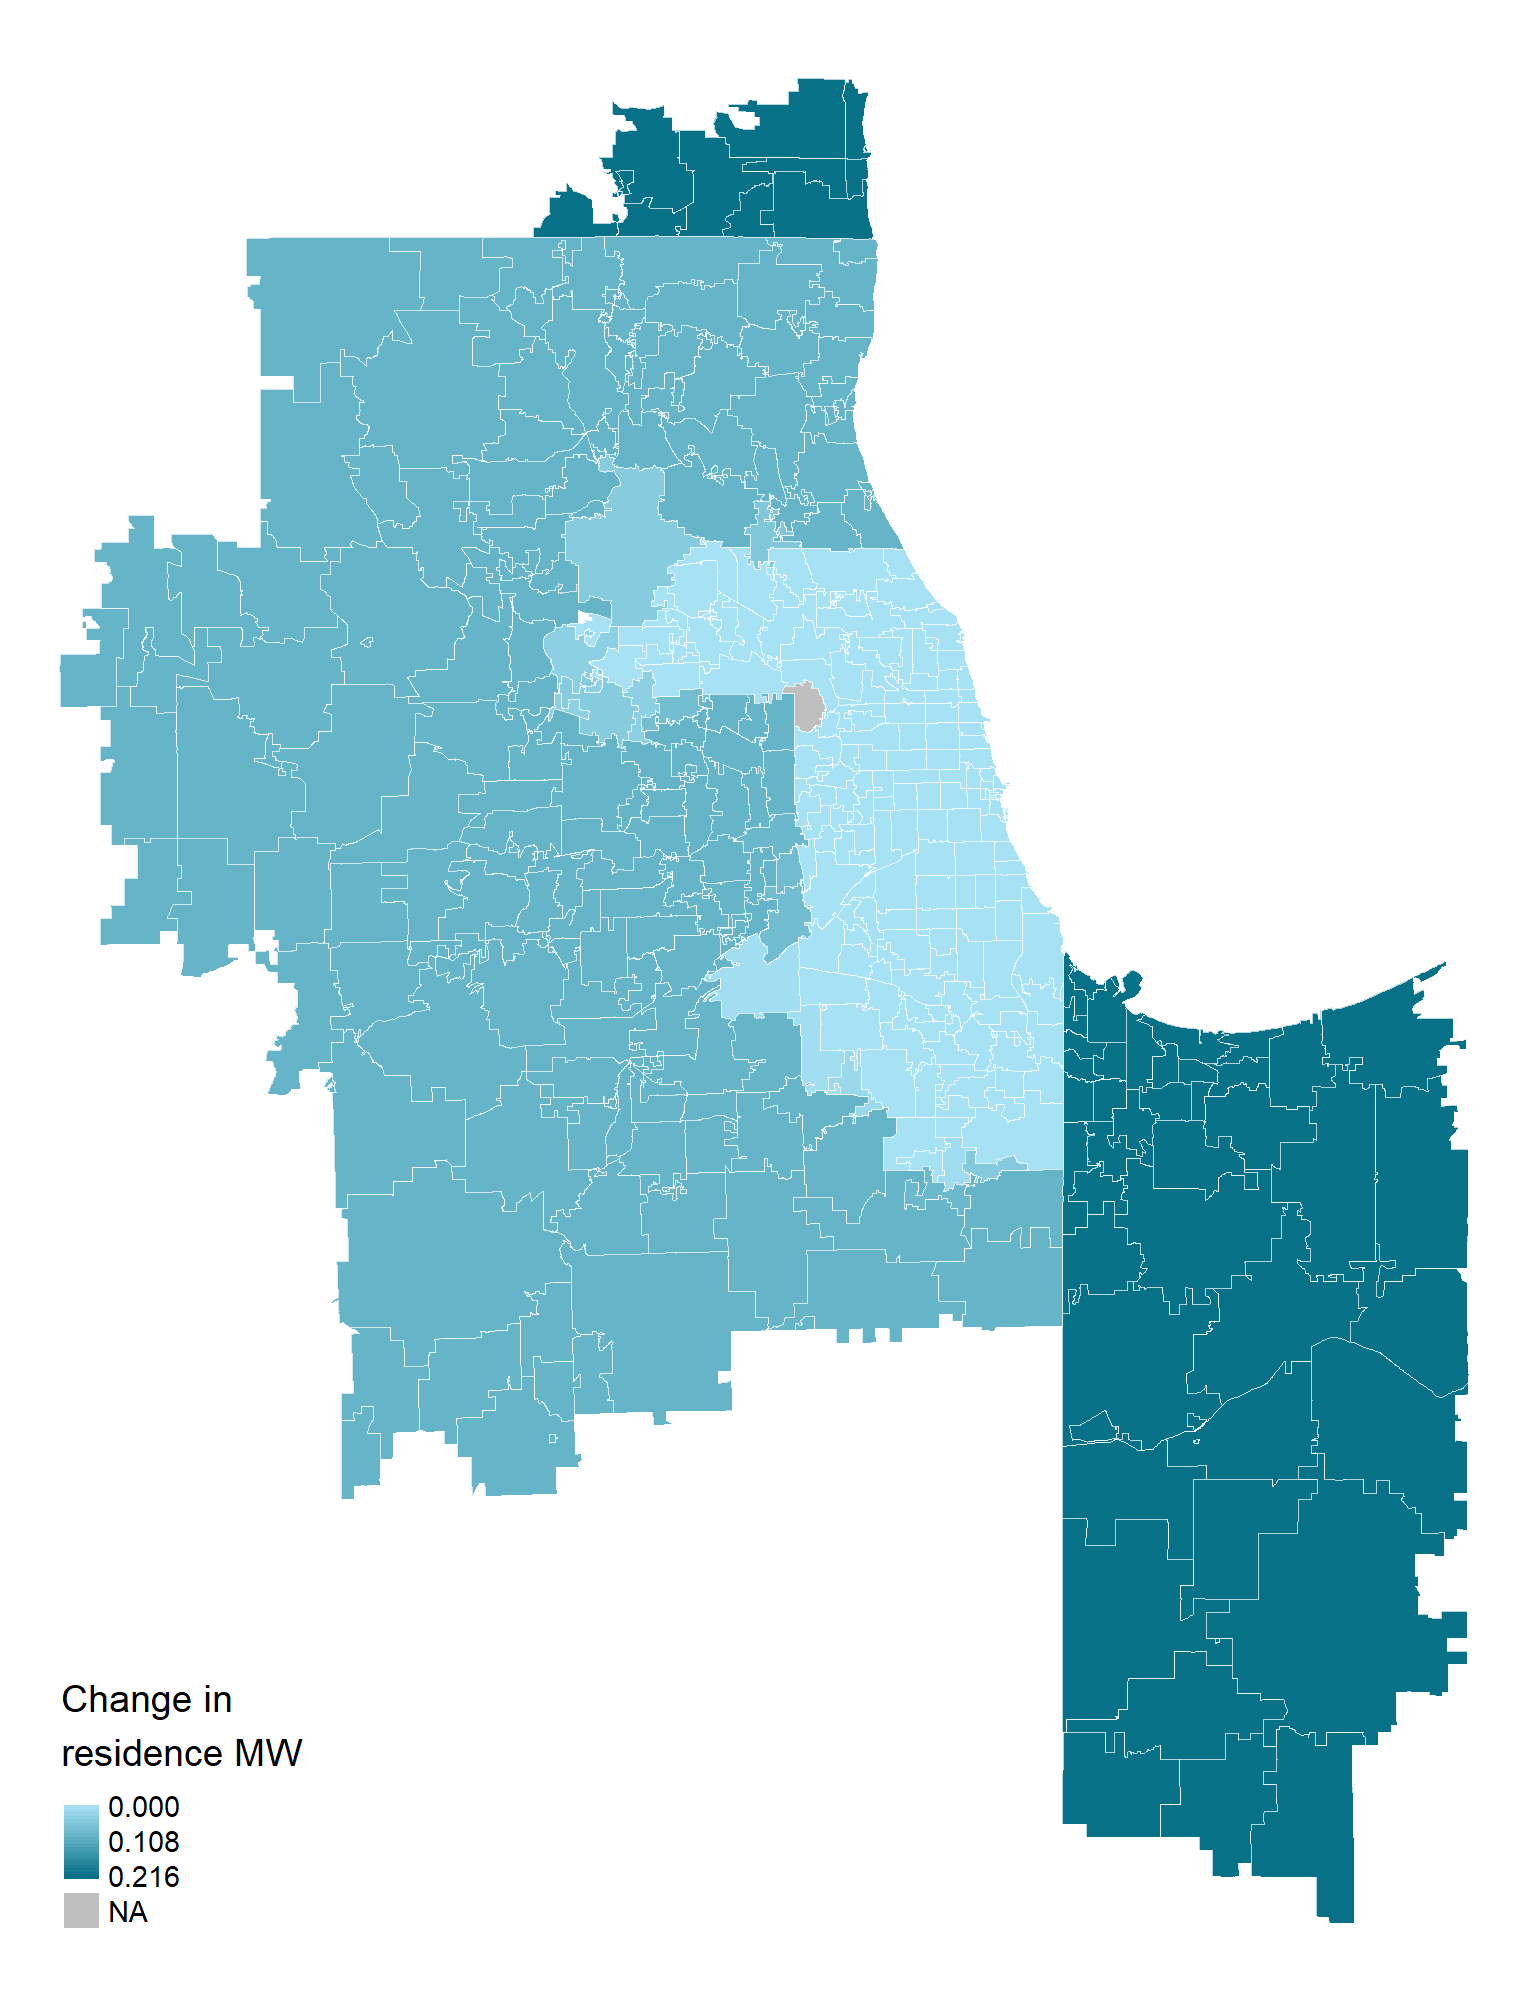
\includegraphics[width = 1\textwidth]
            {counterfactuals/output/chicago_d_mw_res_fed_9usd.png}
    \end{subfigure}%
    $\quad\quad\quad\quad$%
    \begin{subfigure}{.4\textwidth}  \centering
        \caption*{Changes in workplace MW}
        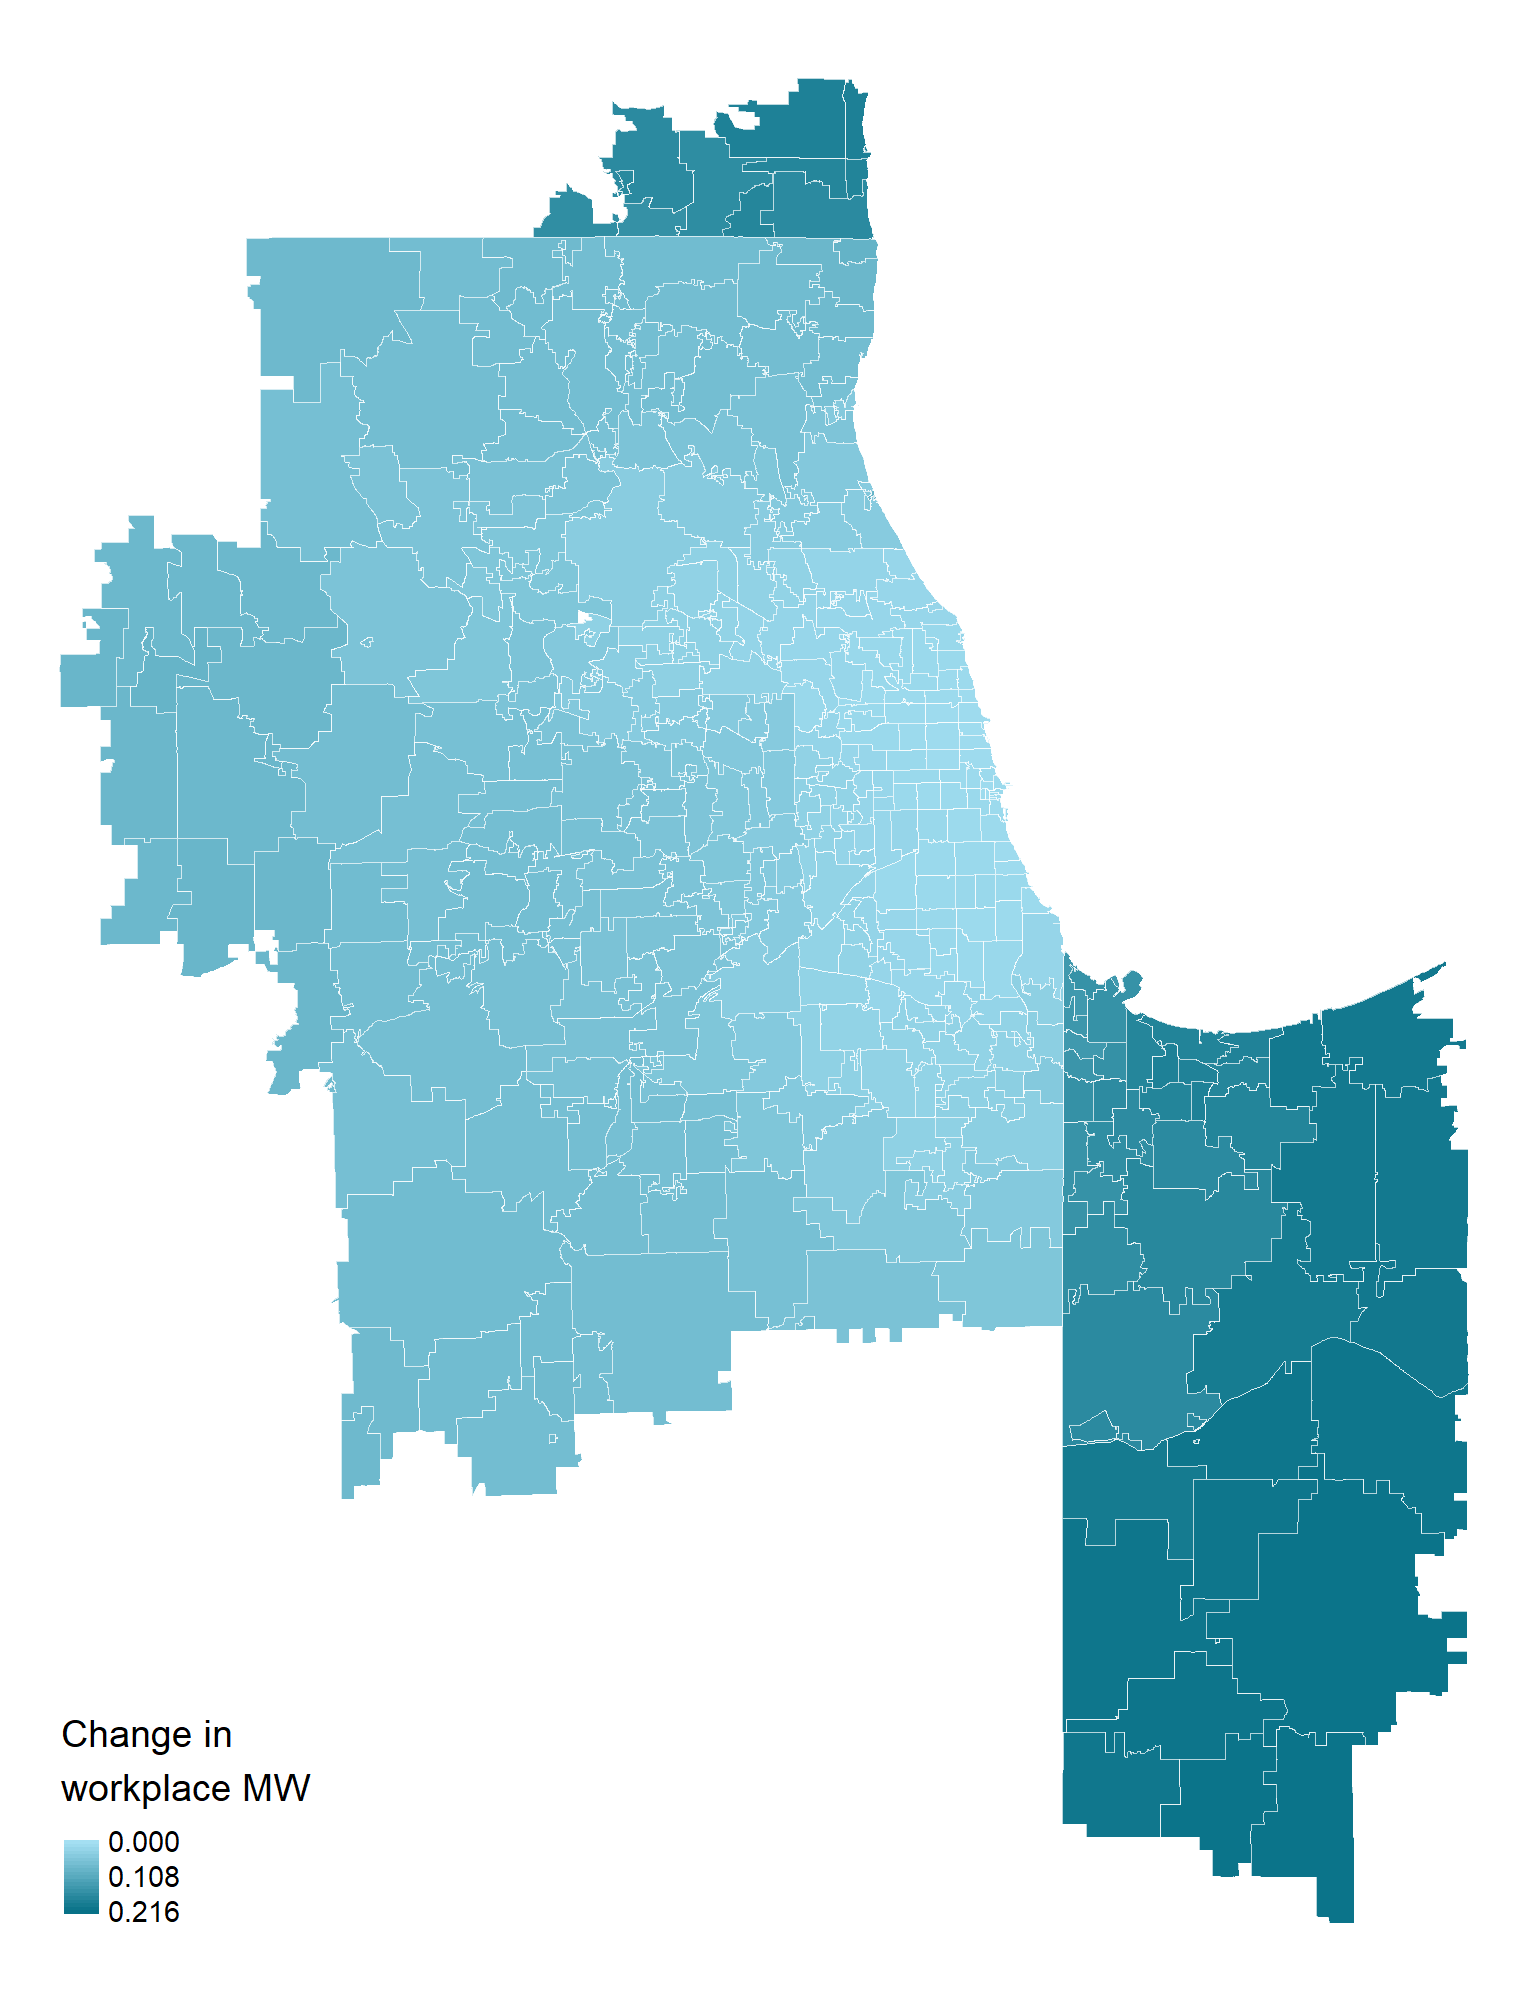
\includegraphics[width = 1\textwidth]
            {counterfactuals/output/chicago_d_mw_wkp_fed_9usd.png}
    \end{subfigure}

    \begin{minipage}{.95\textwidth} \centering
        \vspace{2mm}
        Panel B: Increase in Chicago MW from \$13 to \$14
        \vspace{1.5mm}
    \end{minipage}

    \begin{subfigure}{.4\textwidth}  \centering
        \caption*{Changes in residence MW}
        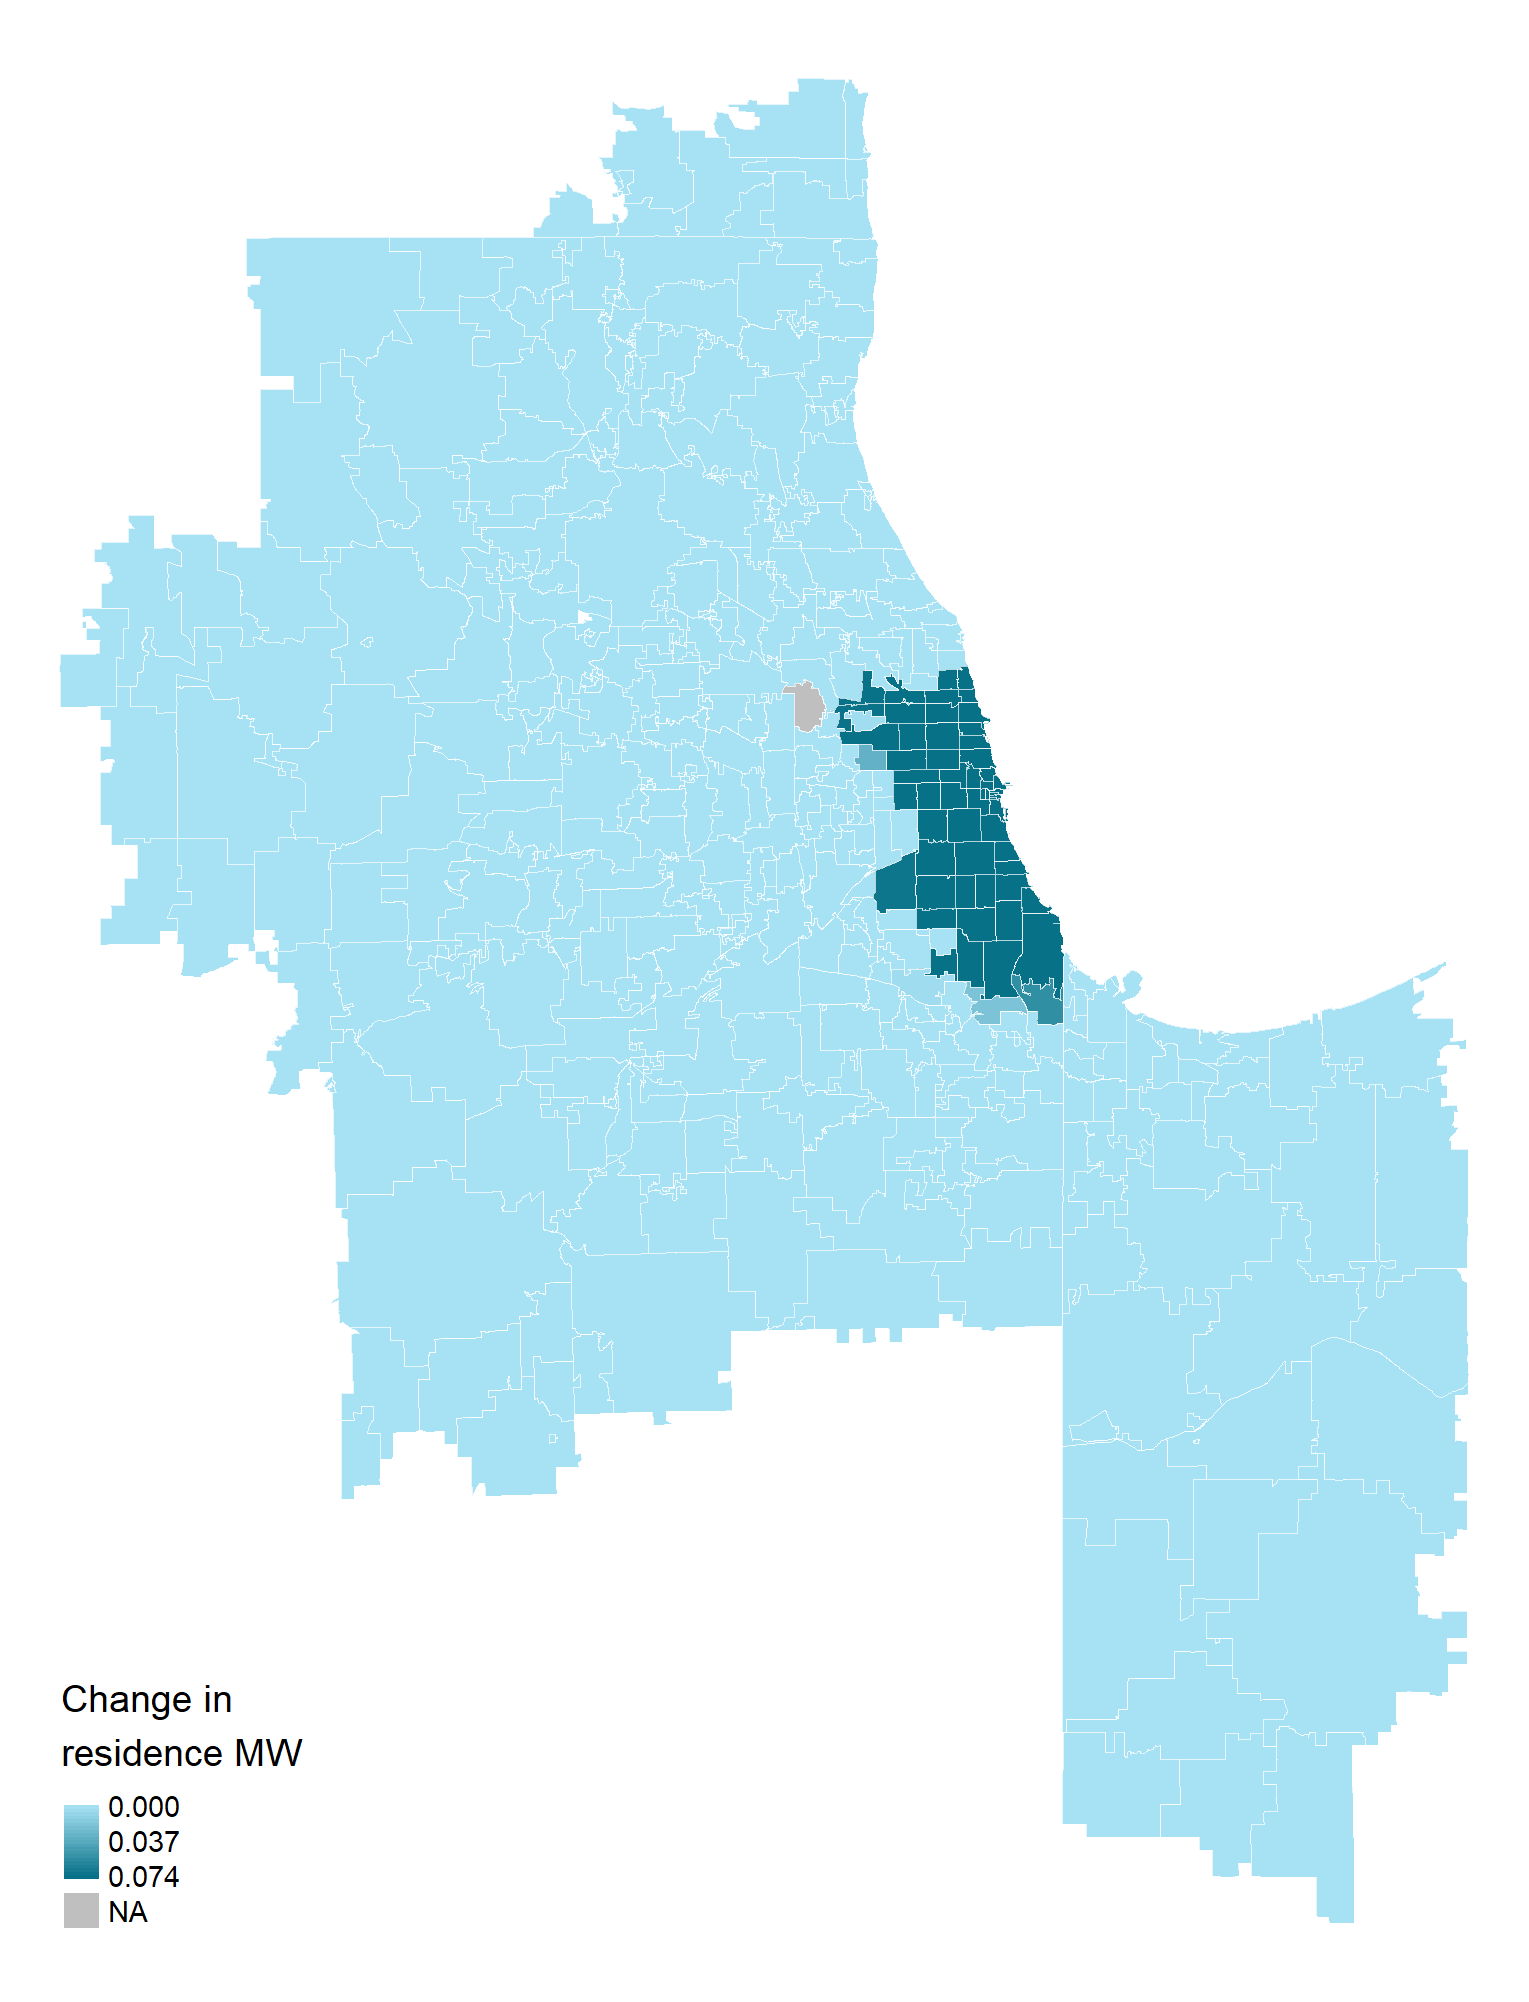
\includegraphics[width = 1\textwidth]
            {counterfactuals/output/chicago_d_mw_res_chi14.png}
    \end{subfigure}%
    $\quad\quad\quad\quad$%
    \begin{subfigure}{.4\textwidth}  \centering
        \caption*{Changes in workplace MW}
        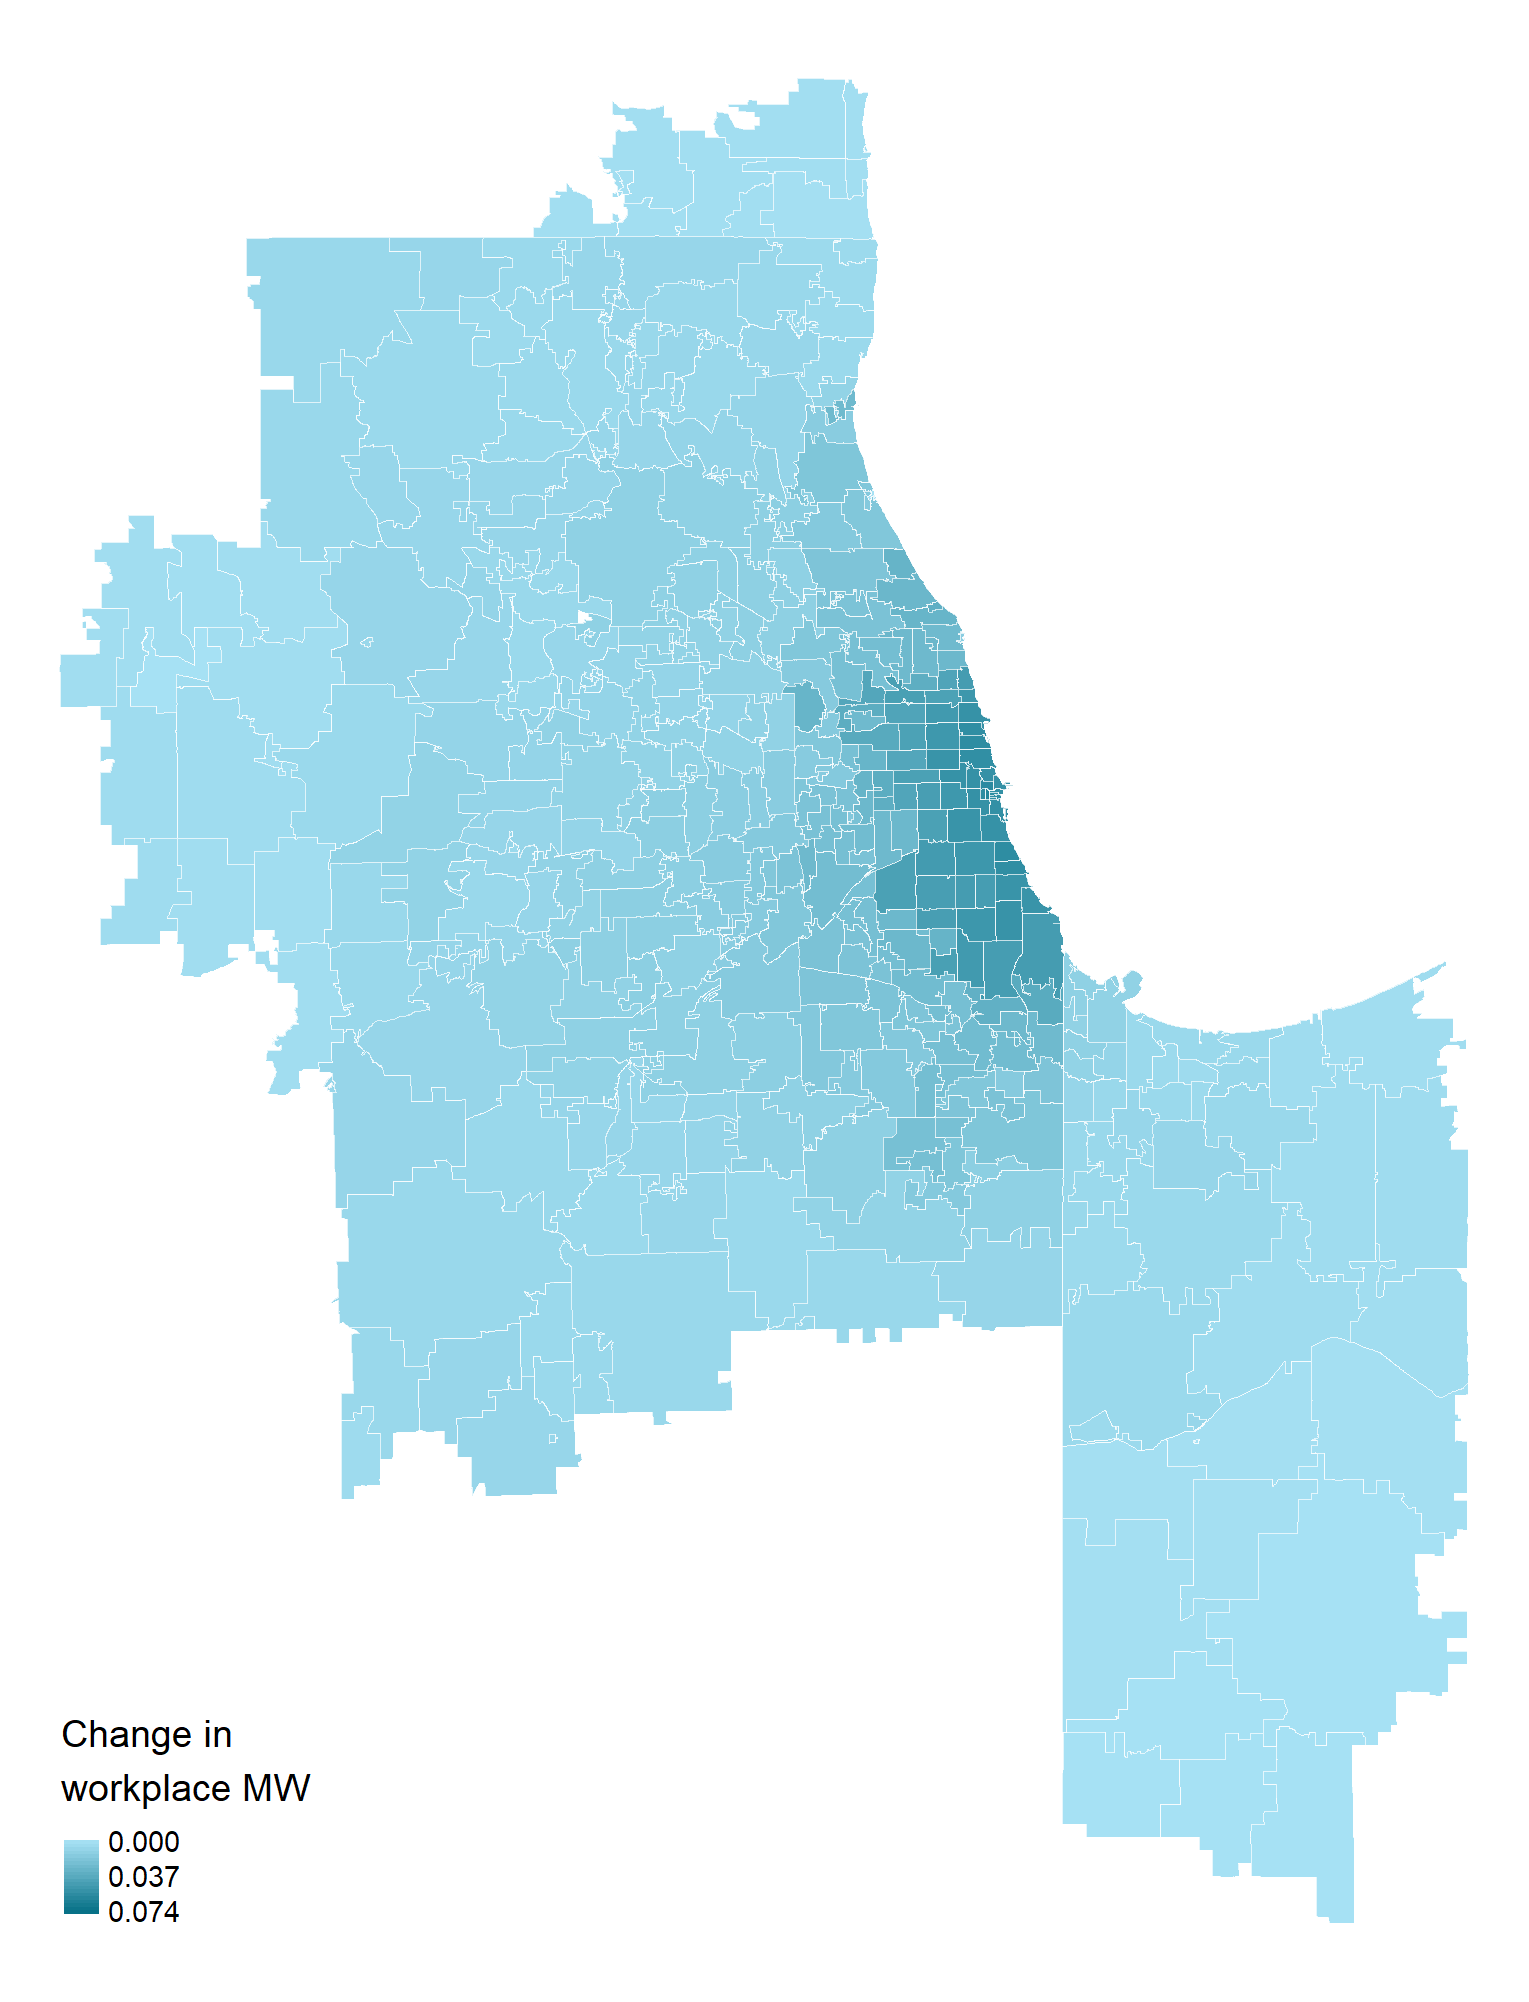
\includegraphics[width = 1\textwidth]
            {counterfactuals/output/chicago_d_mw_wkp_chi14.png}
    \end{subfigure}

    \begin{minipage}{.95\textwidth} \footnotesize
        \vspace{2.5mm}
        Notes:
        Data are from the MW panel described in Section \ref{sec:data_mw_panel} 
        and from LODES.
        The figures map changes in the residence and workplace MW measures 
        by counterfactual MW policies in the Chicago-Naperville-Elgin CBSA.
        Panel A shows a policy where the federal MW increases from \$7.25 to \$9 
        in January 2020, holding constant other MW policies at their December 
        2019 levels.
        Panel B shows a policy where the city of Chicago increases its MW 
        from \$13 to \$14 in January 2020, holding constant other MW policies 
        at their December 2019 levels as well.
    \end{minipage}
\end{figure}
